\section{Результаты измерений}
Параметры установки:

\begin{gather*}
    R=114{,}6\pm 0{,}5\,\text{мм}
    \;\text{(}\varepsilon_R\approx 0{,}004\text{)} \\
    r=30{,}2\pm 0{,}3\,\text{мм} 
    \;\text{(}\varepsilon_r\approx 0{,}01\text{)} \\
    m_0 = 956{,}7\pm 0{,}5\,\text{г}
    \;\text{(}\varepsilon_m\approx 0{,}0005\text{)} \\
    z_0 = 2152\pm 1{,}5\,\text{мм}
    \;\text{(}\varepsilon_{z_0}\approx 0{,}0007\text{)} \\
    g = 9{,}8155\pm 0{,}0005\,\text{м}/\text{с}^2
    \;\text{(}\varepsilon_g\approx 0{,}00005\text{)}
\end{gather*}

\[k=\left(0{,}4\pm 0{,}006\right)\cdot 10^{-3}\,\text{м}^2\text{с}^{-2}
\;\text{(}\varepsilon_k\approx 0{,}015\text{)}\]

\[\varepsilon_I=\varepsilon_m+\varepsilon_k+2\varepsilon_T\]

При измерениях можно пренебречь погрешностью измерений времени, т.к. систематическая
погрешность составляет $5\,\text{мс}$ при измеряемых промежутках примерно в $60\,\text{с}$,
а случайная погрешность мала по сравнению с $0{,}015$ из-за большой массы подвеса (поэтому
трение почти не замедляет его) и большого $z_0$ по сравнению с $R$ и $r$ (поэтому малы
скорости и амплитуды и период колебаний почти не зависит от амплитуды).

Параметры цилиндра:
\begin{gather*}
    m_1 = 772{,}1\pm 0{,}5\,\text{г} \\
    d_1 = 158{,}8\pm 0{,}05\,\text{мм}
\end{gather*}

Параметры диска:
\begin{gather*}
    m_2 = 584{,}7\pm 0{,}5\,\text{г} \\
    d_2 = 170{,}4\pm 0{,}05\,\text{мм}
\end{gather*}

Измерим по 30 колебаний для разных комбинаций грузов.
\begin{itemize}
    \item Без тел: $t_0=122{,}622\,\text{с}$
    \item Цилиндр: $t_1=120{,}560\,\text{с}$
    \item Диск: $t_2=109{,}816\,\text{с}$
    \item Диск и цилиндр: $t_3=113{,}004\,\text{с}$
\end{itemize}

Момент иннерции платформы
\[I_0 = \left(6{,}39\pm 0{,}1\right)\cdot 10^{-3}\,\text{кг}\cdot\text{м}^2
\;\text{(}\varepsilon_{I_0}\approx 0{,}016\text{)}\]
Момент иннерции платформы с цилиндром
\[I_1 = \left(11{,}16\pm 0{,}18\right)\cdot 10^{-3}\,\text{кг}\cdot\text{м}^2
\;\text{(}\varepsilon_{I_1}\approx 0{,}016\text{)}\]
Момент иннерции платформы с диском
\[I_2 = \left(8{,}41\pm 0{,}14\right)\cdot 10^{-3}\,\text{кг}\cdot\text{м}^2
\;\text{(}\varepsilon_{I_2}\approx 0{,}017\text{)}\]
Момент иннерции платформы с диском и цилиндром
\[I_3 = \left(13{,}13\pm 0{,}22\right)\cdot 10^{-3}\,\text{кг}\cdot\text{м}^2
\;\text{(}\varepsilon_{I_3}\approx 0{,}017\text{)}\]

Момент иннерции цилиндра
\[I_c = I_1-I_0 = \left(4{,}77\pm 0{,}28\right)\cdot 10^{-3}\,\text{кг}\cdot\text{м}^2
\;\text{(}\varepsilon_{I_c}\approx 0{,}06\text{)}\]
Теоретическое значение
\[I_{ct} = m_1\left(\frac{d_1}{2}\right)^2 = \left(4{,}867\pm 0{,}006\right)\cdot 10^{-3}\,\text{кг}\cdot\text{м}^2
\;\text{(отклонение эксперимента от теории $2\,\%$)}\]

Момент иннерции диска
\[I_d = I_2-I_0 = \left(2{,}02\pm 0{,}24\right)\cdot 10^{-3}\,\text{кг}\cdot\text{м}^2
\;\text{(}\varepsilon_{I_d}\approx 0{,}11\text{)}\]
Теоретическое значение
\[I_{dt} = \frac{1}{2}m_2\left(\frac{d_2}{2}\right)^2 = \left(2{,}122\pm 0{,}003\right)\cdot 10^{-3}\,\text{кг}\cdot\text{м}^2
\;\text{(отклонение эксперимента от теории $5\,\%$)}\]

Момент иннерции диска и платформы
\[I_{cd} = I_3-I_0 = \left(6{,}73\pm 0{,}32\right)\cdot 10^{-3}\,\text{кг}\cdot\text{м}^2
\;\text{(}\varepsilon_{I_{cd}}\approx 0{,}05\text{)}\]
Теоретическое значение
\[I_{cdt} = I_{dt} + I_{ct} = \left(6{,}990\pm 0{,}009\right)\cdot 10^{-3}\,\text{кг}\cdot\text{м}^2
\;\text{(отклонение эксперимента от теории $4\,\%$)}\]

\[I_c + I_d  = \left(6{,}79\pm 0{,}52\right)\cdot 10^{-3}\,\text{кг}\cdot\text{м}^2\]

\[1 - \frac{I_{cd}}{I_c+I_d}\approx 8\cdot 10^{-3}\]

Аддитивность момента иннерции выполняется с хорошей точностью.

Убедимся в справедливости теоремы Гюйгенса-Штейнера. Для этого придвинем вплотную два
бруска, образующих цилиндр и изменяя расстояние между их серединами $2h$, будем измерять
период 30 колебаний $t_30$. Если в координатах $T^2(h^2)$ точки лягут на прямую, теорема
будет выполнена.

\begin{table}[!ht]
    \centering
    \caption{Зависимость периода 30 колебаний от $h$}
    \begin{tabular}{|l|l|}
    \hline
        $h,\,\pm 0{,}2\,\text{см}$ & $t_{30},\text{с}$ \\ \hline
        0 & 92.395 \\ \hline
        0.5 & 93.161 \\ \hline
        1 & 94.038 \\ \hline
        1.5 & 94.372 \\ \hline
        2 & 96.208 \\ \hline
        2.5 & 98.146 \\ \hline
        3 & 99.669 \\ \hline
        3.5 & 102.434 \\ \hline
        4 & 104.254 \\ \hline
        4.5 & 106.417 \\ \hline
        5 & 110.252 \\ \hline
        5.5 & 113.689 \\ \hline
        6 & 116.311 \\ \hline
        6.5 & 120.030 \\ \hline
        7 & 123.869 \\ \hline
        7.5 & 128.324 \\ \hline
    \end{tabular}
\end{table}

Погрешности измерения времени очень малы, поэтому не учитываются.

Диаметр диска, который образуют грузы $d=12{,}56\pm 0{,}005\,\text{см}$.

\begin{gather*}
    I=kmT^2 \\
    I_0+m\left(\frac{d^2}{8}+h^2+x^2\right)=k\left(m+m_0\right)T^2 \\
    b + x^2 = k\left(1+\frac{m_0}{m}\right)T^2 \\
    b + x^2 = aT^2 \\
    m = \frac{m_0}{\frac{1}{kK}-1} 
\end{gather*}

\begin{figure}[ht!]
    \centering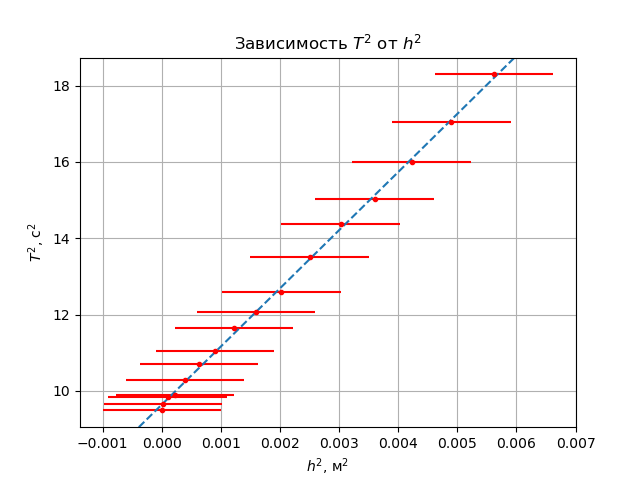
\includegraphics[width=0.8\linewidth]{img/cool-plot.png}
\end{figure}

По МНК $a=1525\pm 13\,\text{с}^2/\text{м}^2$.
\[m=1496\pm 23\,\text{г}\;\text{(взвешивание даёт $1536{,}3\,\text{г}$, ошибка $3\%$)}\]
\[I=k(m_0+m)T(0)^2-I_0=\left(2{,}91\pm 0{,}09\right)\cdot 10^{-3}\,\text{кг}\cdot\text{м}^2\]
теоретическое значение $3{,}03\cdot 10^{-3}\,\text{кг}\cdot\text{м}^2$, ошибка $4\,\%$.

Проведём аналогичные измерения для смещения в направлении, перпендикулярном рёбрам брусков.
$2h$~--- расстояние между торцами брусков.

\begin{table}[!ht]
    \centering
    \caption{Зависимость периода 30 колебаний от $h$}
    \begin{tabular}{|l|l|}
    \hline
        $h,\,\pm 0{,}2\,\text{см}$ & $t_{30},\text{с}$ \\ \hline
        0 & 92.433 \\ \hline
        0.5 & 94.583 \\ \hline
        1 & 97.059 \\ \hline
        1.5 & 99.721 \\ \hline
        2 & 102.367 \\ \hline
        2.5 & 106.43 \\ \hline
        3 & 109.910 \\ \hline
        3.5 & 113.010 \\ \hline
        4 & 116.953 \\ \hline
        4.5 & 120.367 \\ \hline
        5 & 125.733 \\ \hline
        5.5 & 130.315 \\ \hline
        6 & 134.548 \\ \hline
        6.5 & 137.253 \\ \hline
    \end{tabular}
\end{table}

Формулы для массы и момента иннерции будут аналггичны предыдущим.

\begin{figure}[ht!]
    \centering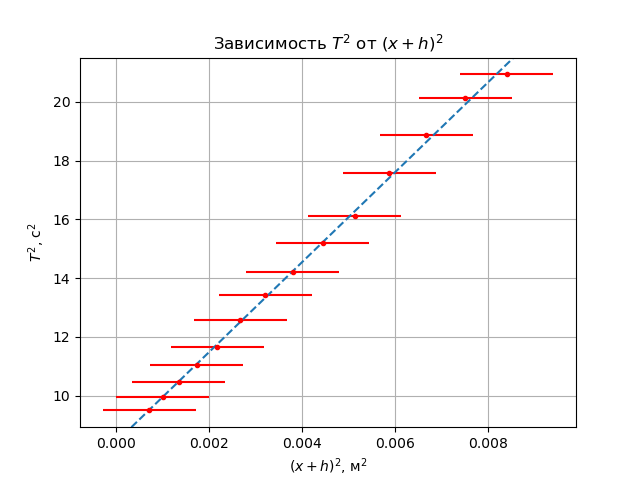
\includegraphics[width=0.8\linewidth]{img/fucking-plot.png}
\end{figure}

По МНК $a=1532\pm 17\,\text{с}^2/\text{м}^2$.
\[m=1512\pm 39\,\text{г}\;\text{(взвешивание даёт $1536{,}3\,\text{г}$, ошибка $2\%$)}\]
\[I=k(m_0+m)T(0)^2-I_0=\left(2{,}97\pm 0{,}12\right)\cdot 10^{-3}\,\text{кг}\cdot\text{м}^2\]
теоретическое значение $3{,}03\cdot 10^{-3}\,\text{кг}\cdot\text{м}^2$, ошибка $2\,\%$.

Точки легли на прямую, поэтому теорема Гюйгенса-Штейнера выполняется.
